%==============================================================================
% Programação Linear III
% 18/08/2021
%==============================================================================

\chapter{Programação Linear III}

\section{Nomenclatura e Notação} %---------------------------------------------

Considere o problema de P.L. $ \min z = cx $ sujeito a $ Ax = b $, $ x \geq 0 $.

Aqui já foram introduzidas as variáveis de folga e de excesso.
E sobre a matriz $ A $, as hipóteses de sempre: $ A $ é $ m \times n $ de 
\textit{rank} $ m $.
O problema está na forma padrão.

O que vamos apresentar aqui são os preparativos para aplicação do 
\textbf{Algorítimo Simplex} e discussão da \textit{solução ótima}.

Como foi visto na parte \texttt{Programação Linear II}, dado o conjunto $ I $, a
solução básica fica identificada e o conjunto $ J $ também.

Suponha que se tenha uma solução básica factível $I$ de 

\begin{align*}
  \min \quad        & z = cx \\
  \text{s.a.} \quad & 
                      \begin{aligned}[t]
                        Ax &= b \\
                         x &\geq 0  
                      \end{aligned}
\end{align*}

Paralelamente, para facilitar o entendimento, expressemos o problema na forma 
escalar.

\begin{align*}
  \min \quad       & z = \custoGeral{n} \\
  \text{s.a} \quad & 
                     \begin{aligned}[t]
                       \linhaSistema{1} &= b_1 \\
                       \linhaSistema{2} &= b_2 \\
                                        &\vdots \\
                       \linhaSistema{m} &= b_m
                     \end{aligned}\\
                   & x_1, x_2, \dots, x_n \geq 0
\end{align*}

Então, $ c = \begin{bmatrix} c_1 & c_2 & \ldots & c_n \end{bmatrix} $ e 
$ x^{t} = \begin{bmatrix} x_1 & x_2 & \ldots & x_n \end{bmatrix} $.

\[
  A = \begin{bmatrix}
        a_{11} & a_{12} & \ldots & a_{1n} \\
        a_{21} & a_{22} & \ldots & a_{2n} \\
        \vdots & \vdots & \ddots & \vdots \\
        a_{m1} & a_{22} & \ldots & a_{mn} \\
      \end{bmatrix}
  \qquad
  \text{ e }
  \quad
  b = \begin{bmatrix}
        b_1 \\ 
        b_2 \\ 
        \vdots \\ 
        b_m
      \end{bmatrix}
\]

Vejamos a notação em termos dos conjuntos $ I $ e $ J $.
\[
  c = \begin{bmatrix}
        c_{I} & c_{J}
      \end{bmatrix},
  \qquad
  x = \begin{bmatrix}
        x_{I} \\
        x_{J}
      \end{bmatrix}
  \qquad
  \text{ e }
  \qquad
  A = \begin{bmatrix}
        A^{I} & A^{J}
      \end{bmatrix}
\]

Em $ c_I $ estão os coeficientes das variávis básicas na F.O. e $ c_J $ os 
coeficientes das variáveis não básicas na F.O.

Em $ x_{I} $ estão as variáveis básicas e em $ x_J $ , as não básicas.

Em $ A^{I} $ estão as colunas da matriz $ A $, correspondentes às variáveis,
cujos índices estão em $ I $ e na mesma  ordem em que aparecem em $ I $.

Em $ A^{J} $ estão as colunas da matriz $ A $ correspondentes às variáveis não
básicas, cujos índices estão em $ J $ e em geral, são colocadas em ordem 
crescente dos índices.

Como já definido em \texttt{Programação Linear II}, $ A^{I} $ é uma matriz 
$ m \times n $ \textit{inversível}, que será denotada por 
$ \left(A^I\right)^{-1} $.

Daqui em diante toda expressão que envolver a matriz $ \left( A^{I} \right)^{-1} $
será denotada com "$\^$" (chapéu).
Os conjuntos $ I $ e $ J $ desempenham papel importante nesta notação e ajudam
na discussão da solução ótima e mais adiante, na \textbf{Análise de Sensibilidade}

\begin{center}
\fbox{
  \begin{minipage}{.9\linewidth}
    \textit{Análise de Sensibilidade} é a discussão sobre o que acontece à 
    solução ótima, se algum dado inicial do problema for alterado e que 
    procedimentos efetuar.
  \end{minipage}
}
\end{center}

Vamos expressar o problema em termos de $ I $ e de $ J $.

\begin{align*}
  \min \quad         & z = \begin{bmatrix} c_I & c_j \end{bmatrix} \begin{bmatrix} x_I\\ x_J \end{bmatrix} \\
  \text{s.a.} \quad & \begin{aligned}[t]
                        \begin{bmatrix}A^I & A^J\end{bmatrix} \begin{bmatrix}x_I \\ x_J\end{bmatrix} &= b \\
                        x_I, x_j &\geq 0
                      \end{aligned}
\end{align*}

Efetuando as operações indicadas obtem-se:

\begin{align*}
  \min \quad        & z = c_Ix_I + c_Jx_J \\
  \text{s.a.} \quad &
                      \begin{aligned}
                        A^{I} x_I + A^{J}x_J &= b \\
                        x_I, x_J &\geq 0
                      \end{aligned}
\end{align*}

O método utilizado pelo Algorítimo Simplex é do \textbf{gradiente reduzido}.
O que será feito agora é multiplicar os dois membros da equação das restrições
por $ \left( A^{I} \right)^{-1} $ para encontrar os valores das variáveis 
básicas ($ x_I $) e substituí-los na F.O.

\begin{align*}
  \min \quad        & z = c_Ix_I + c_Jx_J \\
  \text{s.a.} \quad &
                      \begin{aligned}
                        \textcolor{blue}{\left( A^{I} \right)^{-1}}A^{I} x_I + \textcolor{blue}{\left( A^{I} \right)^{-1}}A^{J}x_J &= \textcolor{blue}{\left( A^{I} \right)^{-1}}b \\
                        x_I, x_J &\geq 0
                      \end{aligned}
\end{align*}

o que resulta:

\begin{align*}
  \min \quad        & z = c_Ix_I + c_Jx_J \\
  \text{s.a.} \quad &
                      \begin{aligned}
                        \mathbb{I} x_I + \left( A^{I} \right)^{-1}A^{J}x_J &= \left( A^{I} \right)^{-1}b \\
                        x_I, x_J &\geq 0
                      \end{aligned}
\end{align*}

ou ainda

\begin{align*}
  \min \quad        & z = c_Ix_I + c_Jx_J \\
  \text{s.a.} \quad &
                      \begin{aligned}
                        x_I + \left( A^{I} \right)^{-1}A^{J}x_J &= \left( A^{I} \right)^{-1}b \\
                        x_I, x_J &\geq 0
                      \end{aligned}
\end{align*}

Assim, $ x_I =  \left( A^{I} \right)^{-1} b - \left( A^{I} \right)^{-1} A^{J} x_J $
que substituindo na F.O., obtém-se:

\begin{align*}
  \min \quad        & z = c_I\left[\left( A^{I} \right)^{-1} b - \left( A^{I} \right)^{-1} A^{J} x_J\right] + c_Jx_J \\
  \text{s.a.} \quad &
                      \begin{aligned}[t]
                        x_I + \left( A^{I} \right)^{-1}A^{J}x_J &= \left( A^{I} \right)^{-1}b \\
                        x_I, x_J &\geq 0
                      \end{aligned}
\end{align*}

Isolando $ x_j $ na F.O., obtém-se:

\begin{align*}
  \min \quad        & z = c_I \left(A^{I}\right)^{-1}b + \left[c_J - c_I\inversaA A^J\right] x_J \\
  \text{s.a.} \quad &
                      \begin{aligned}[t]
                        x_I + \inversaA A^{J} x_J &= \inversaA b \\
                                         x_I, x_J &\geq 0
                      \end{aligned}
\end{align*}

Antes de apresentar a notação simplificada para as expressões, façamos alguns
comentários importantes.

\begin{enumerate}
  \item Note que na F.O. não aparecem as variáveis básicas, ou seja, os 
   coeficientes delas é zero.
  \item A expressão $ c_I \inversaA b $ é uma constante.
  \item Visto que numa \textit{solução básica} as variáveis \textit{não} básicas 
   assumem o valor zero, resulta que o valor de $ z $ em cada solução básica é
   sempre $c_I \inversaA b $ e que os valores das variáveis básicas é 
   $ \inversaA b $.
  \item Note também que se alguma variável não básica assumir algum valor 
   positivo, o valor de $ z $ se altera, desde que o coeficiente dessa variável
   não básica, que assumir um valor positivo, seja diferente de zero.
   Também alterará os valores das variáveis básicas das linhas (equações) em que
   o coeficiente dessa variável não básica  for diferente de zero.
  \item Em $ c_J - c_I\inversaA A^J $ estão todos os coeficientes das variáveis
   não básicas na F.O. e estes podem ser positivos, negativos ou zero.
  \item Em $ \inversaA A^{J} $ estão as colunas que são o coeficientes nas 
   restrições das variáveis não básicas.
   Esses coeficientes podem ser positivos, negativos ou zero.
  \item Por fim, em $ \inversaA b $ estão os valores das variáveis básicas.
\end{enumerate}

Passemos, agora, à notação simplificada.

\[
  \widehat{c}_J = c_J - c_I \inversaA A^J
  \qquad
  \text{ e }  
  \qquad
  \widehat{c}_j = c_j - c_I \inversaA A^j
\]

Logo, 
\[
  \widehat{c}_J = 
  \begin{bmatrix} 
    \widehat{c}_{j_{_1}} & \widehat{c}_{j_{_2}} & \cdots & \widehat{c}_{j_{_{n - m}}}
  \end{bmatrix}
\]

$ \widehat{c}_j $ é o coeficiente da variável $ x_j $, na F.O.

\[
  \widehat{A}^J = \inversaA A^J
  \qquad
  \text{ e }  
  \qquad
  \widehat{A}^j = \inversaA A^{j} 
\]

Note que $ \widehat{A}^j $ é um vetor coluna em que estão os coeficientes da
variável não básica, $ x_j $, nas restrições.

\[
  \widehat{A}^J =
  \begin{bmatrix}
    \widehat{a}_{1j_{_1}} & \widehat{a}_{1j_{_2}} & \cdots & \widehat{a}_{1j_{_{n - m}}} \\
    \widehat{a}_{2j_{_1}} & \widehat{a}_{2j_{_2}} & \cdots & \widehat{a}_{2j_{_{n - m}}} \\ 
    \vdots                & \vdots                & \ddots & \vdots \\
    \widehat{a}_{mj_{_1}} & \widehat{a}_{mj_{_2}} & \cdots & \widehat{a}_{mj_{_{n - m}}}
  \end{bmatrix}
  ,
  \qquad
  \widehat{A}^j =
  \begin{bmatrix}
    \widehat{a}_{1j} \\
    \widehat{a}_{2j} \\
    \vdots \\
    \widehat{a}_{mj} 
  \end{bmatrix}
\]
bem como,
$
  \widehat{b} = \inversaA b = 
    \begin{bmatrix}
      \widehat{b}_1 \\
      \widehat{b}_2 \\
      \vdots \\
      \widehat{b}_m \\
    \end{bmatrix}
$

Outros elementos que aparecerão na discussão da solução ótima são a 
\textbf{equação de bloqueio}, que fornece as informações de que variável básica
sairá da base e o valor com que a variável não básica entrará na base.

\[
  x_I + \widehat{A}^j x_j = \widehat{b},
\]

e o cálculo prático extraído da equação de bloqueio para obter essas informações.

\[ 
  \min 
  \left\{ 
    \frac{\widehat{b}_i}{\widehat{a}_{ij}};\quad \widehat{a}_{ij} > 0.
  \right\}
\]

Analisemos a equeação de bloqueio.
Expressemo-la em mais detalhes de acordo com o que foi exposto acima.

\[
  \begin{bmatrix}
    x_{B_{_1}} \\
    x_{B_{_2}} \\
    \vdots     \\
    x_{B_{_m}} 
  \end{bmatrix}  
  +
  \begin{bmatrix}
    a_{ij} \\
    a_{2j} \\
    \vdots \\
    a_{mj}
  \end{bmatrix}
  =
  \begin{bmatrix}
    b_{1}  \\
    b_{2}  \\
    \vdots \\
    b_{m}
  \end{bmatrix}
\]

Note que se todos os $ \widehat{a}_{ij} \leq 0 $, nenhuma variável básica,
$ x_{B_{i}} $, tende a zero, se $ x_j $ aumentar de valor.
Se algum $ \widehat{a}_{ij} > 0 $, então a variável básica da mesma linha, 
$ x_{B_{i}} $ tende a zero.
E qual é o valor atingido por $ x_j $ que torna $ x_{B_i} $ zero?
É exatamente o quociente 

\[
  \frac{\widehat{b}_i}{\widehat{a}_{ij}}
\]

Se houver mais de um $ \widehat{a}_{ij} > 0 $, então as correspondentes variáveis
básicas tenderão a zero, quando $ x_j $ aumentar de valor.
Como nenhuma variável pode ser negativa, $ x_j $ só pode aumentar de valor até
a primeira variável básica atingir o valor zero.

No caso em que todos os $ \widehat{a}_{ij} \leq 0 $, o que a equação de bloquio
representa?

Note que $ \widehat{A}^{j} $ é um vetor \ldots 

$ \widehat{b} $ é outro vetor fixo, constante\ldots

A equação representa um raio de origem  em $ \widehat{b} $ e direção 
$ \widehat{A}^j $.
Aqui $ x_j $ faz o papel do $ \lambda $ e $ x_I $, o papel do ponto que descreve
o raio.

Veja a Figura~\ref{fig:vetor}

\begin{figure}[!h]
  \centering
  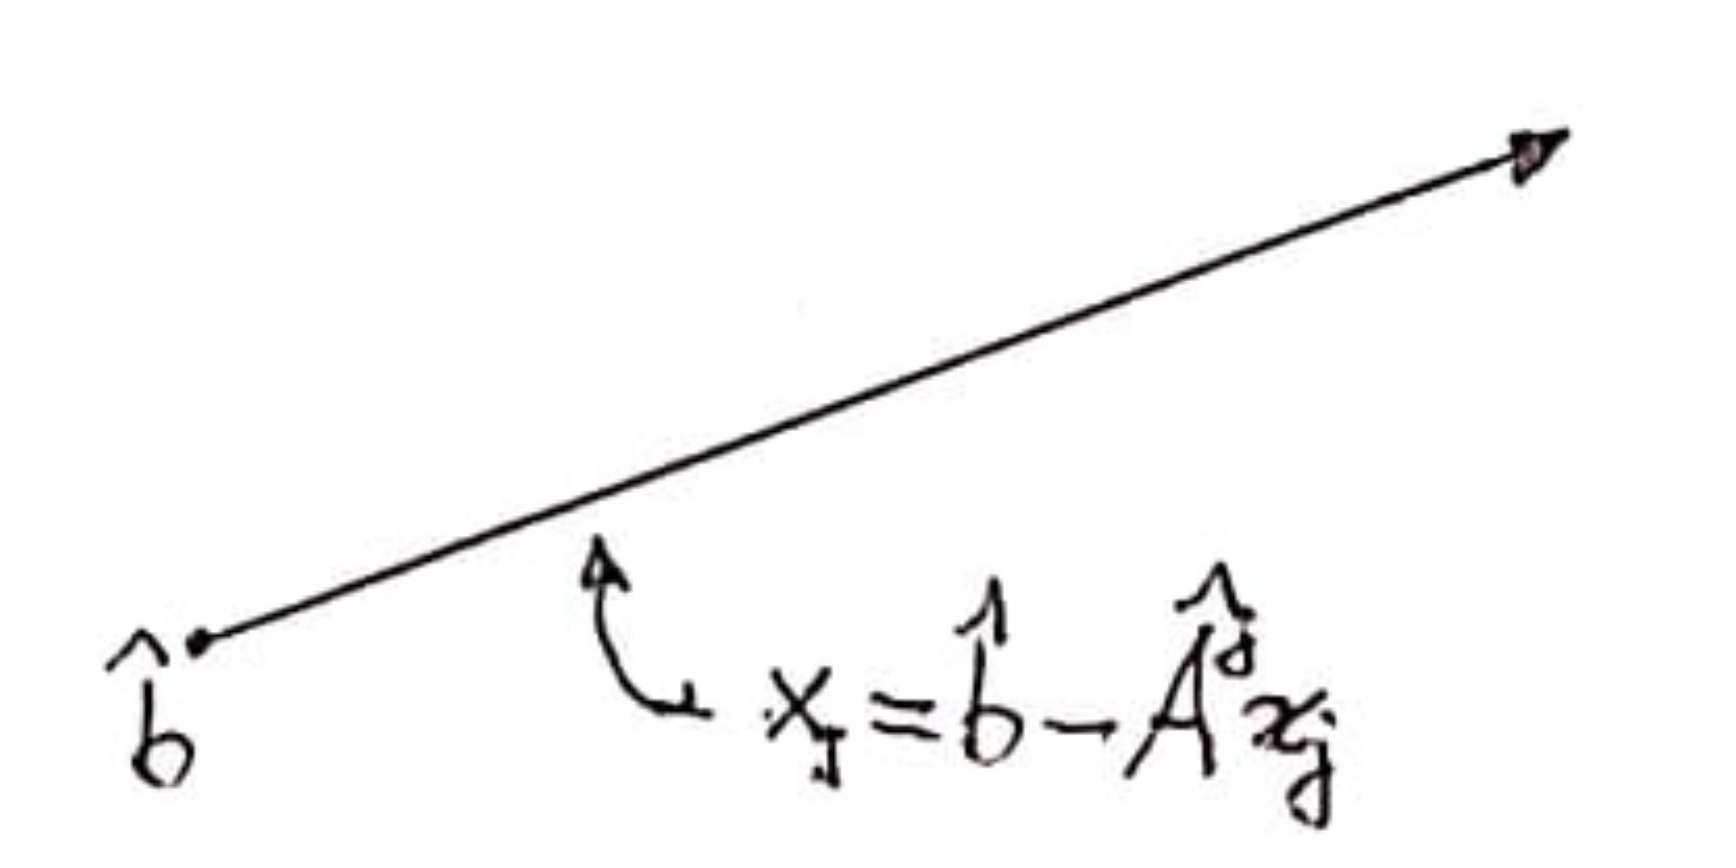
\includegraphics[width = 0.8\linewidth]{vetor.png}
  \caption{}
  \label{fig:vetor}
\end{figure}

\newpage

Mas, lembrando que se o conjunto das soluções $ Ax = b $, $ x \geq 0 $ é limitado,
não tem raio nem direção; tem arestas.
Se é ilimitado tem arestas que são raios.
Veja a Figura~\ref{fig:planos}.

\begin{figure}[!h]
  \centering
  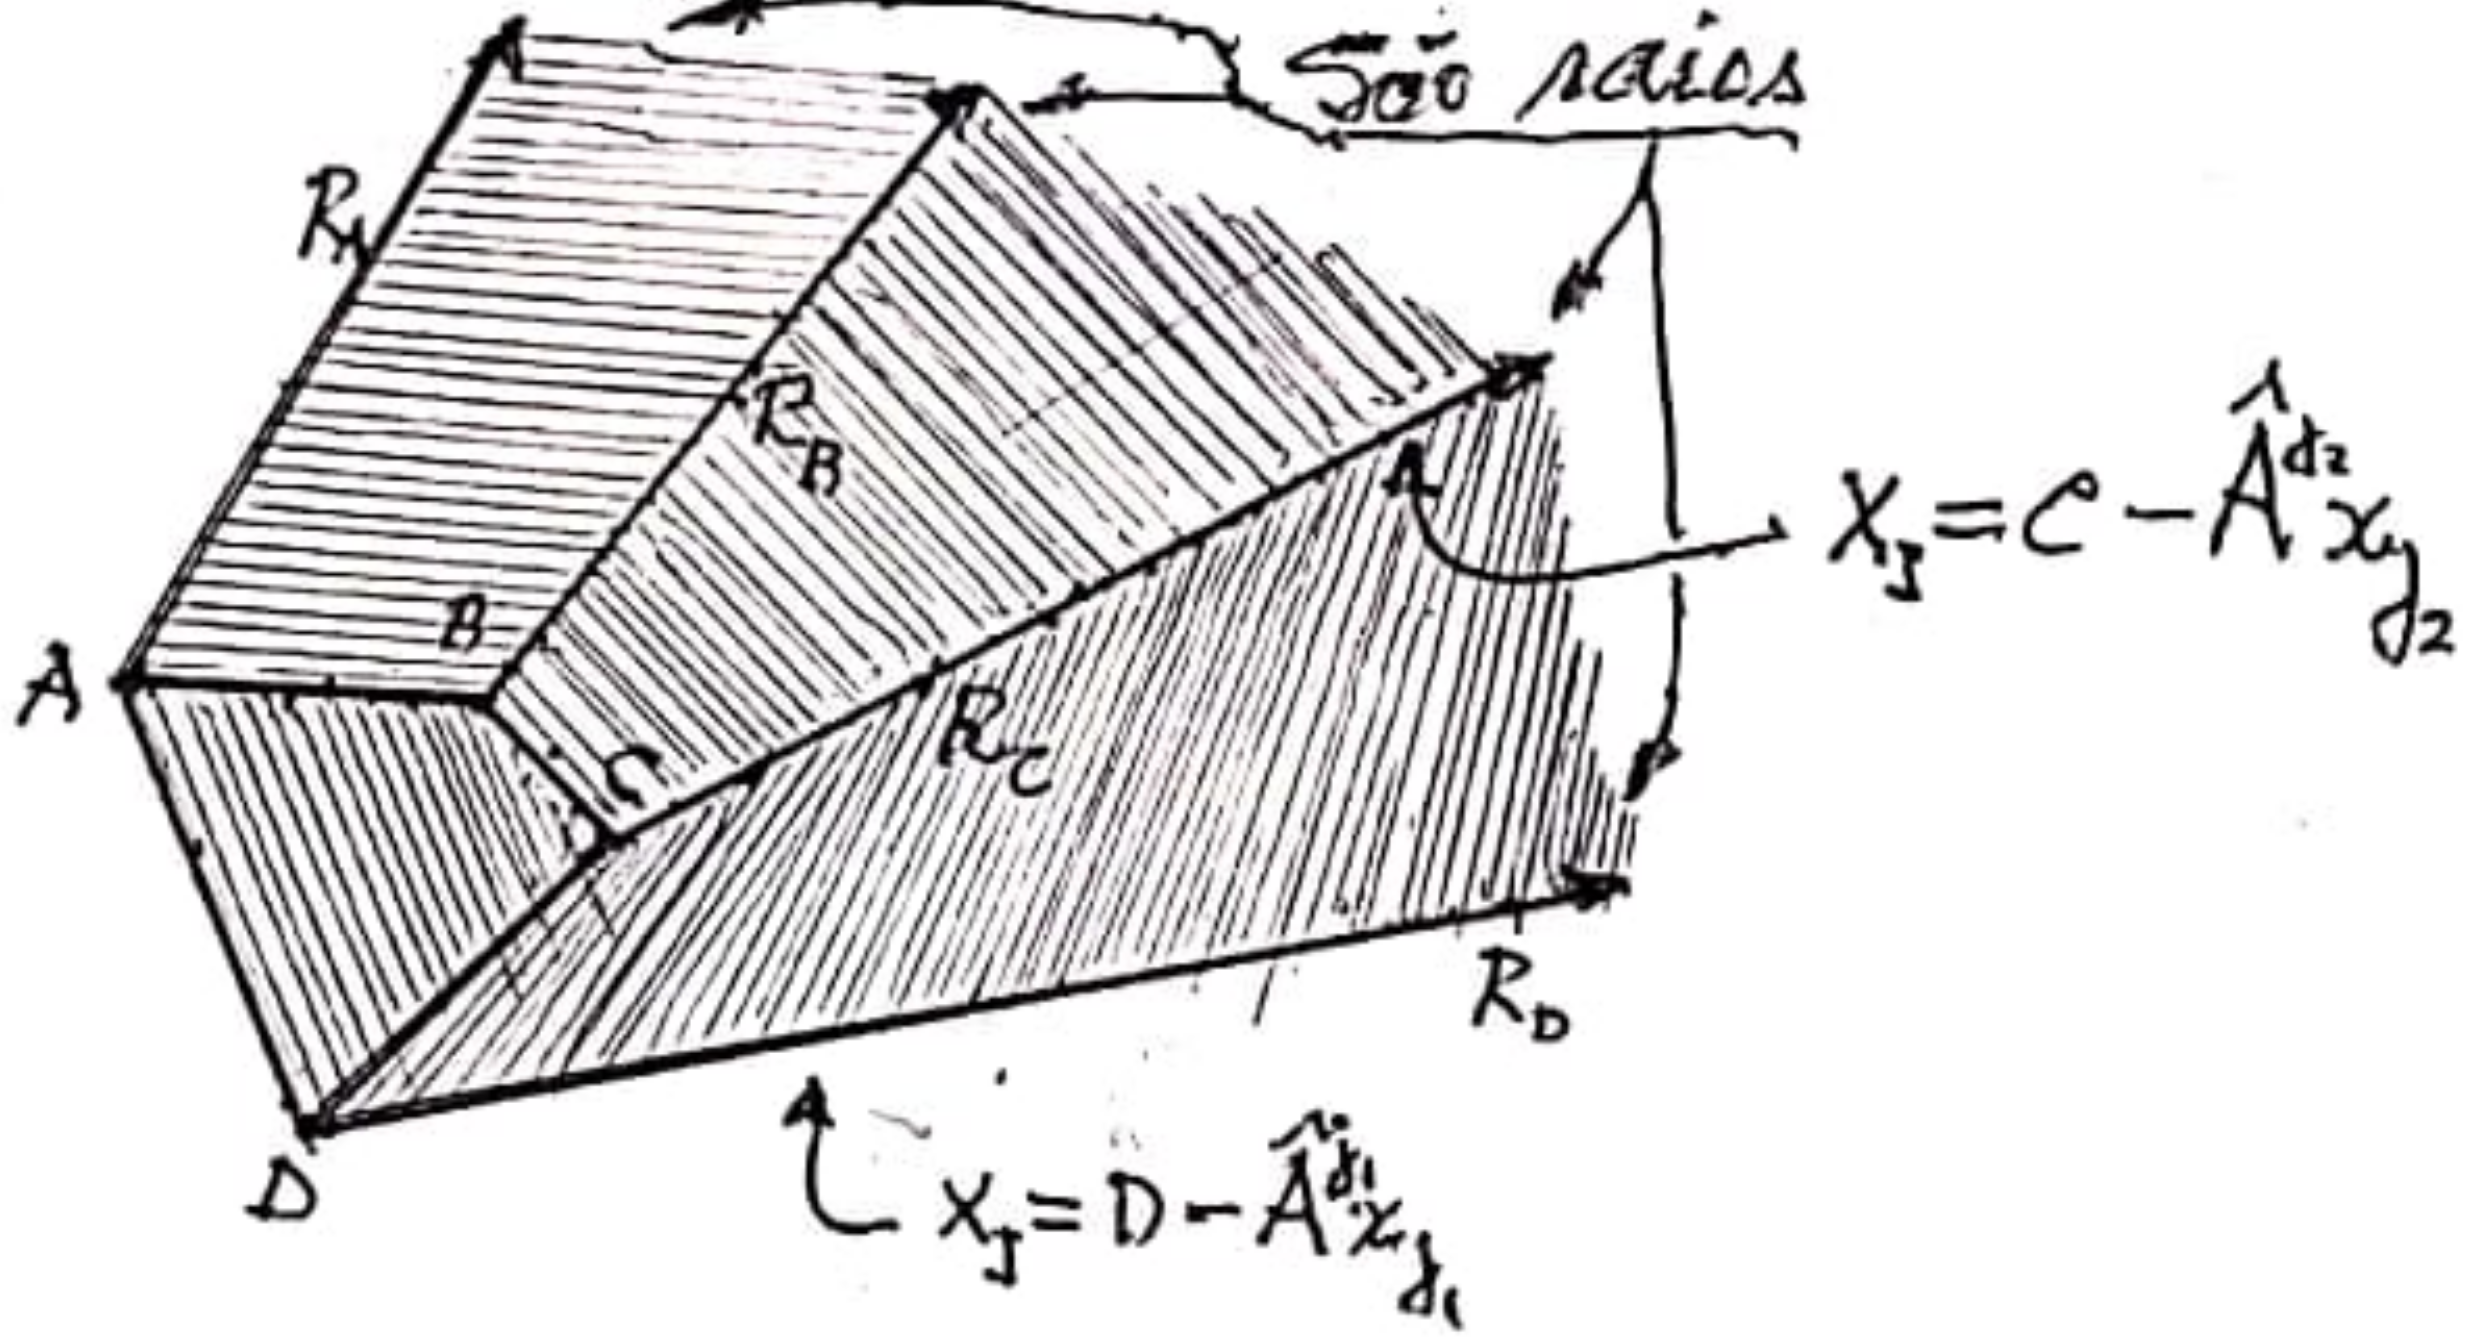
\includegraphics[width = \linewidth]{belo_desenho.png}  
  \caption{}
  \label{fig:planos}
\end{figure}

$ A, B, C \text{ e } D $ são pontos extremos, há oito arestas das quais quatro
são raios com origens em $ A, B, C \text{ e } D $.
Denominamos esses raios, respectivamente, por $ R_A, R_B, R_C \text{ e } R_D $.
O politopo é a interseção de cinco semiespaços, que são representados por cinco
inequações.
São elas:

\begin{enumerate}
  \item A que contém os pontos $ A $ e $ D $ e os pontos dos raios $ R_A $ e 
    $ R_D $.
    É a face invisível pela posição mostrada;
  \item A que contém os pontos $ A $ e $ B $ e os pontos dos raios $ R_A $ e
    $ R_B $;
  \item A que contém os pontos $ B $ e $ C $ e os pontos dos raios $ R_B $ e 
    $ R_C $;
  \item A que contém os pontos $ C $ e $ D $ e os pontos dos raios $ R_C $ e 
  $ R_D $;
  \item A que contém os pontos $ A, B, C \text{ e } D $.
\end{enumerate}

Cada inequação tem três variáveis, o que indica que após introduzir  as variáveis
de folga e de excesso obtém-se um sistema de cinco equações e oito variáveis.

Se, por exemplo, a solução atual for o ponto extremo $ C $, a variável candidata
para entrar na base seja $ x_j $ é $ \widehat{A}^j \leq 0 $, significa que ao
aumentar o valor de $ x_j $, nenhuma variável básica irá para zero.
As soluções vão percorrendo o raio $ R_C $.
Se algum $ \widehat{a}_{ij} > 0 $, então a solução percorrerá a aresta que vai
para $ B $ ou $ D $.

Se o conjunto das soluções de $ Ax = b $, $ x \geq 0 $ é \textbf{limitado}, este
não tem direção, logo, não tem raio.
Veja a Figura~\ref{fig:tetraedro}.

\begin{figure}[!h]
  \centering
  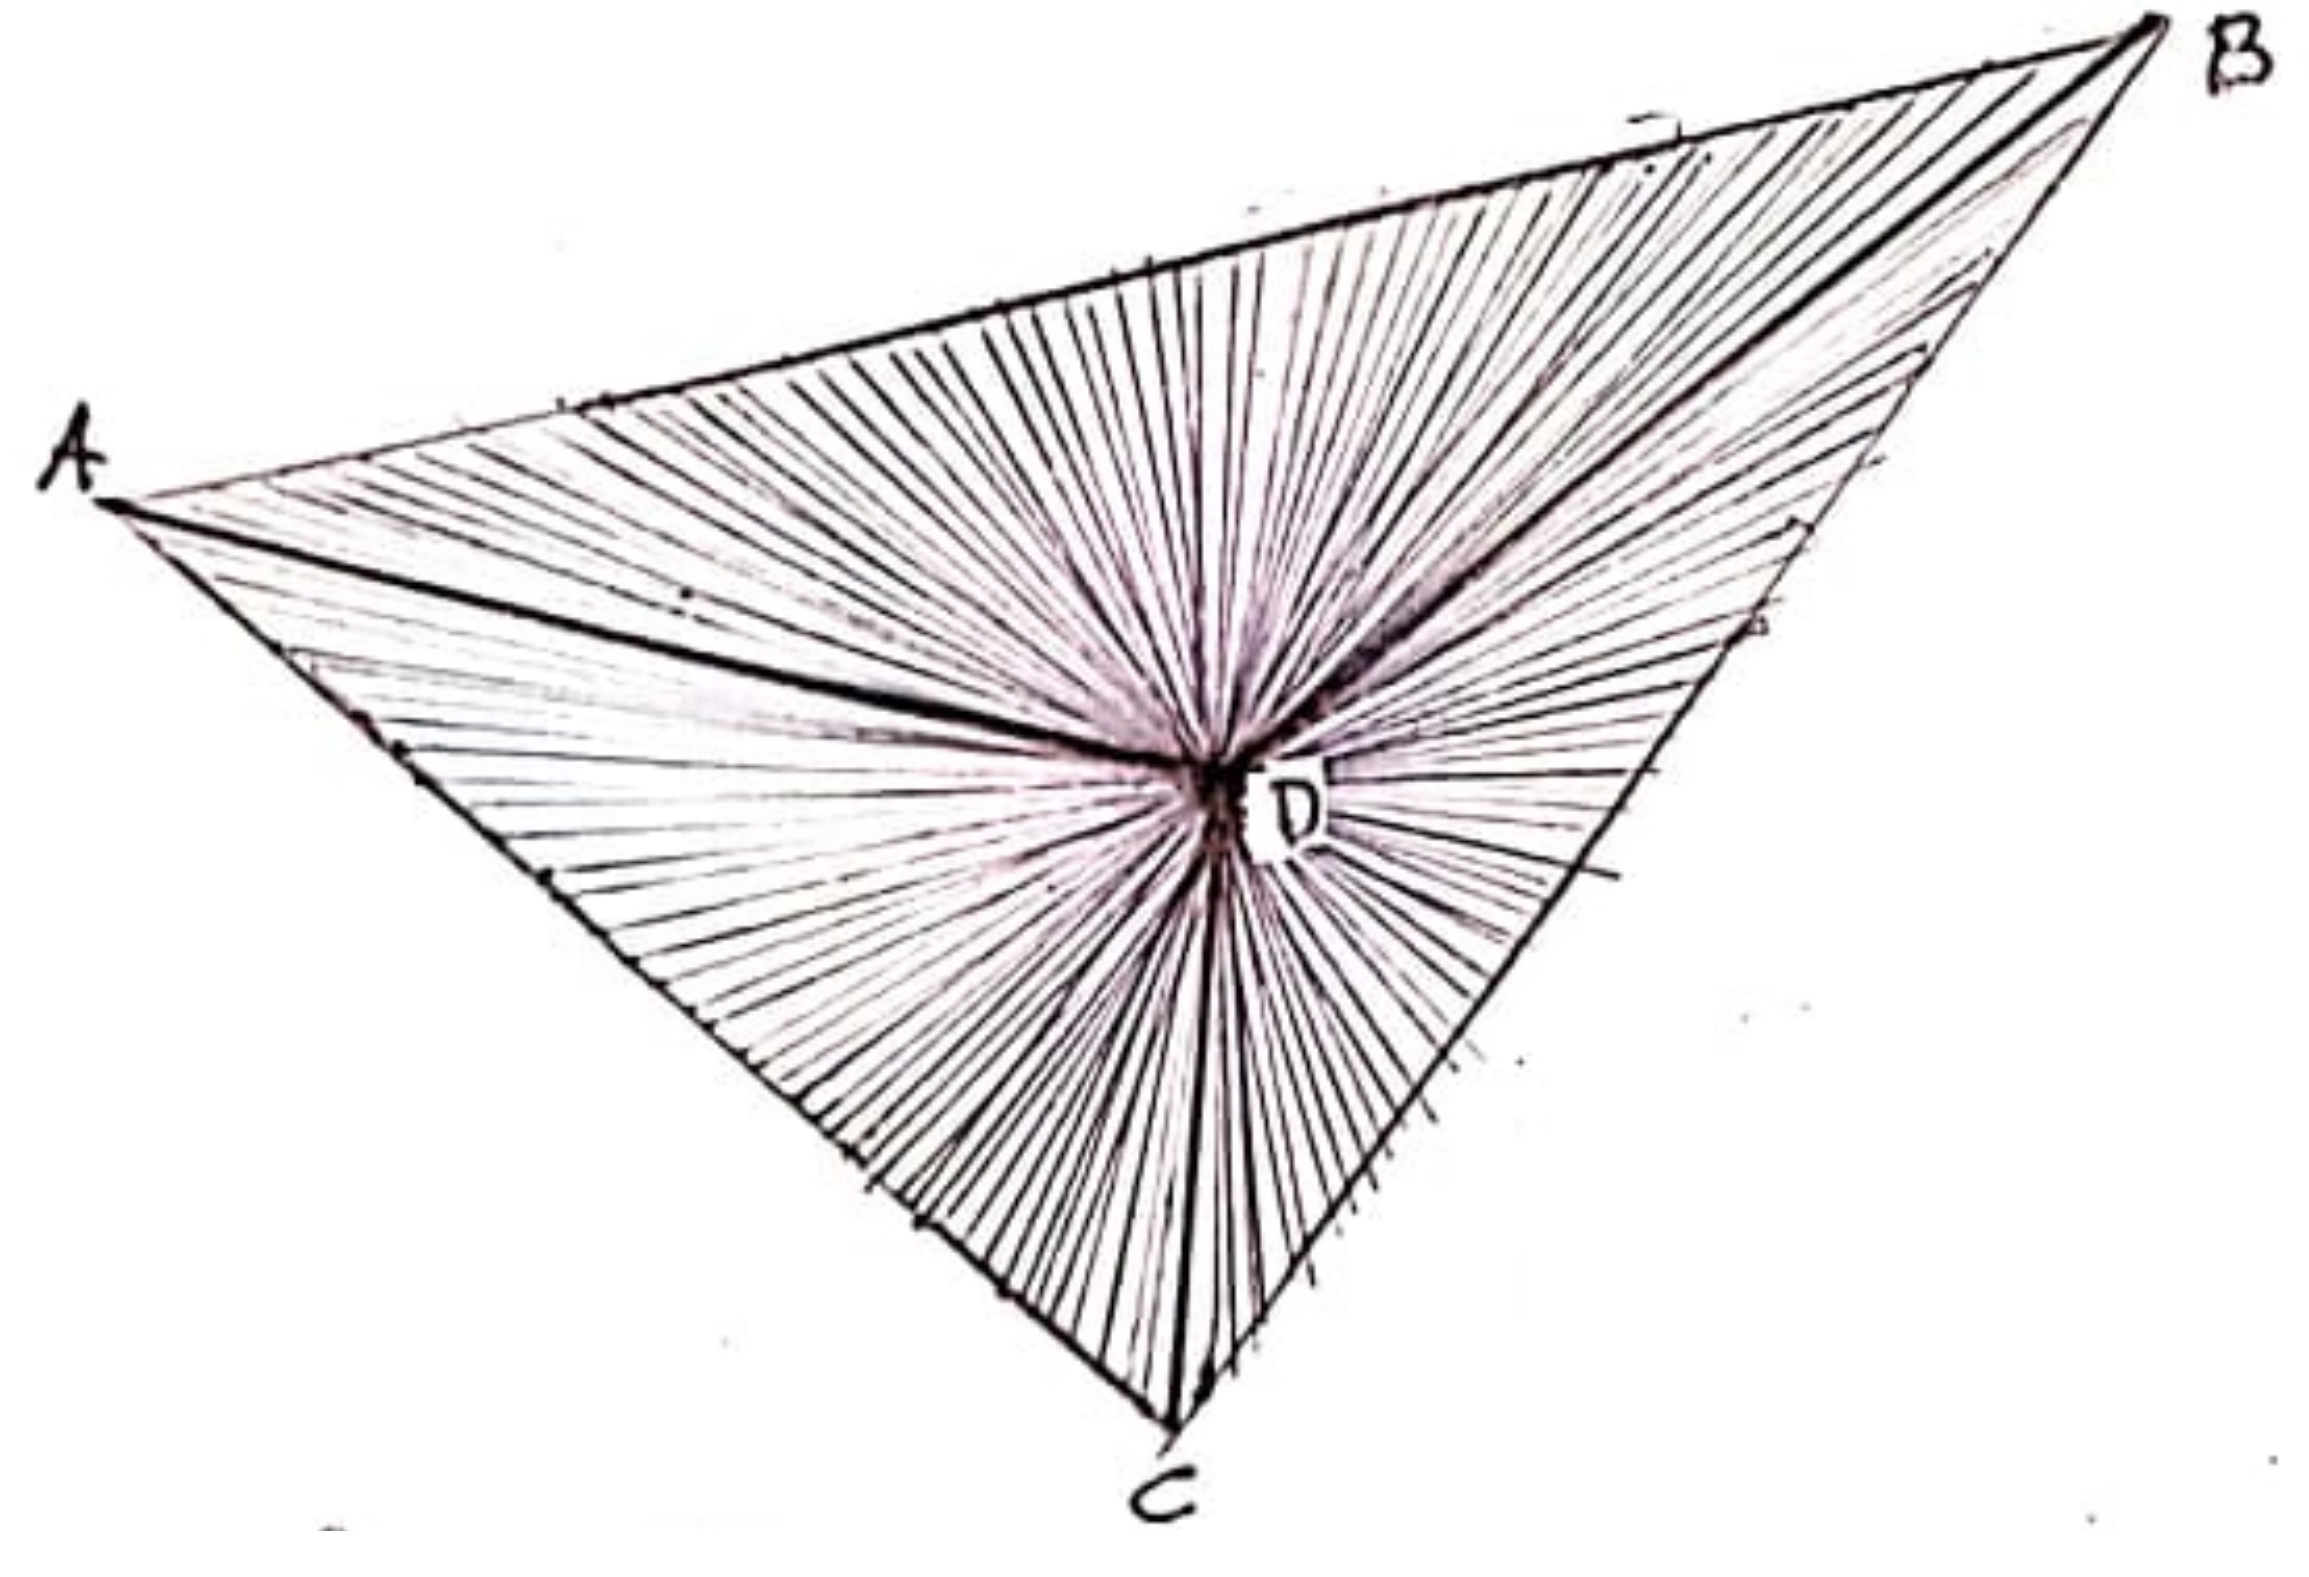
\includegraphics[width = 0.8\linewidth]{tetraedro.png}  
  \caption{Um tetraedro visto de cima}
  \label{fig:tetraedro}
\end{figure}

Os vértices $ A, B, C $ e $ D $ são pontos extremos.
Cada face correspondente a um plano e cada plano é definido pelos trios de pontos:
$ ABC, ABD, ACD \text{ e } BCD $.
O tetraedro é a interseção dos quatro semiespaços, em que pelo menos uma inequação
é do tipo "$ \geq $" e no máximo três.
A generalização para acontecer a Figura~\ref{fig:tetraedro} é:

\[
  \begin{cases}
    a_1x_1 + a_2x_2 + a_3x_3 &\leq \alpha_1 \\
    b_1x_1 + b_2x_2 + b_3x_3 &\stackrel[\leq]{\geq}{\phantom{=}} \alpha_2 \\
    c_1x_1 + c_2x_2 + c_3x_3 &\stackrel[\leq]{\geq}{\phantom{=}} \alpha_3 \\
    d_1x_1 + d_2x_2 + d_3x_3 &\leq \alpha_4 
  \end{cases}
\]

Note que esse politopo não tem direção.
Se $ d $ é um vetor não nulo e $ x_0 $ um ponto qualquer do politopo, para algum\\
$ \lambda > 0 $ o ponto $ x = x_0 + \lambda d $ não vai satisfazer o sistema  
acima.
Em outras palavras, o ponto $ x $ não pertencerá ao politopo.

Uma observação sobre os exemplos dados acima é que o espaço considerado é o 
$ \mathbb{R}^3 $.
As Figuras \ref{fig:planos} e \ref{fig:tetraedro} podem estar no espaço 
$ \mathbb{R}^{4} $, $ \mathbb{R}^{5} $, etc.
Como foi dito que eram resultados de interseção de inequações com três variáveis,
então poderiam estar no $ \mathbb{R}^{3}, \mathbb{R}^{4}, \mathbb{R}^{5} $, 
\ldots, qualquer um.
O número de variáveis diz qual é a dimensão \textit{mínima} do espaço em que 
essas inequações estão inseridas.
Então, ao ser apresentada uma equação ou uma inequação, deve ser dito em que 
espaço estão inseridas.
Por exemplo:

\begin{exemplo}
  O que representa a equação $ 2x - 5y = 7 $?
\end{exemplo}

Bem\ldots\ depende!
Se for em $ \mathbb{R}^{2} $ é uma \textit{reta}; se for em $ \mathbb{R}^{3} $ é
um \textit{plano}; e, se for em $ \mathbb{R}^{4} $, um \textit{hiperplano}.
A reta tem apenas uma dimensão, enquanto um plano tem duas.
O hiperplano depende da dimensão do espaço em que está inserido.
Por exemplo, a equação $ 3x + 2y - 5z + 7w = 4 $ não pode ser um plano.
Há aí, pelo menos, três variáveis livres, o que indica que representa um 
hiperplano de, pelo menos, três dimensões.
Por que "pelo menos"?
Se for em $ \mathbb{R}^{4} $, tem dimensão três, mas se for em $ \mathbb{R}^{5} $,
tem dimensão quatro.
O fato da quinta variável não aparecer na equação, diz que ela é uma variável 
livre.
A dimensão é o \textit{número de variáveis livres na equação}, logo, tem que se
dizer (dar) o espaço em que o objeto representado por aquela equação está 
inserido.

E qual a dimensão no caso de inequação?
Ganha mais uma dimensão, pois uma qualquer das variáveis não depende das outras.
Por exemplo, $ 2x + 3y \leq 6 $.
Se $ x = 1 $, $y$ não fica determinado. 
Há uma infinidade de valores que $ y $ pode assumir.
Isso independente de ser em $ \mathbb{R}^{2} $, $ \mathbb{R}^{2} $, \ldots.
Observe que $ 2x + 3y \leq 6 $ em $ \mathbb{R}^{2} $ é o semiespaço, isto é,
uma metade do plano $ \mathbb{R}^{2} $.
Qual é a dimensão?
Dois, é a resposta.

\begin{figure}[!h]
  \centering
  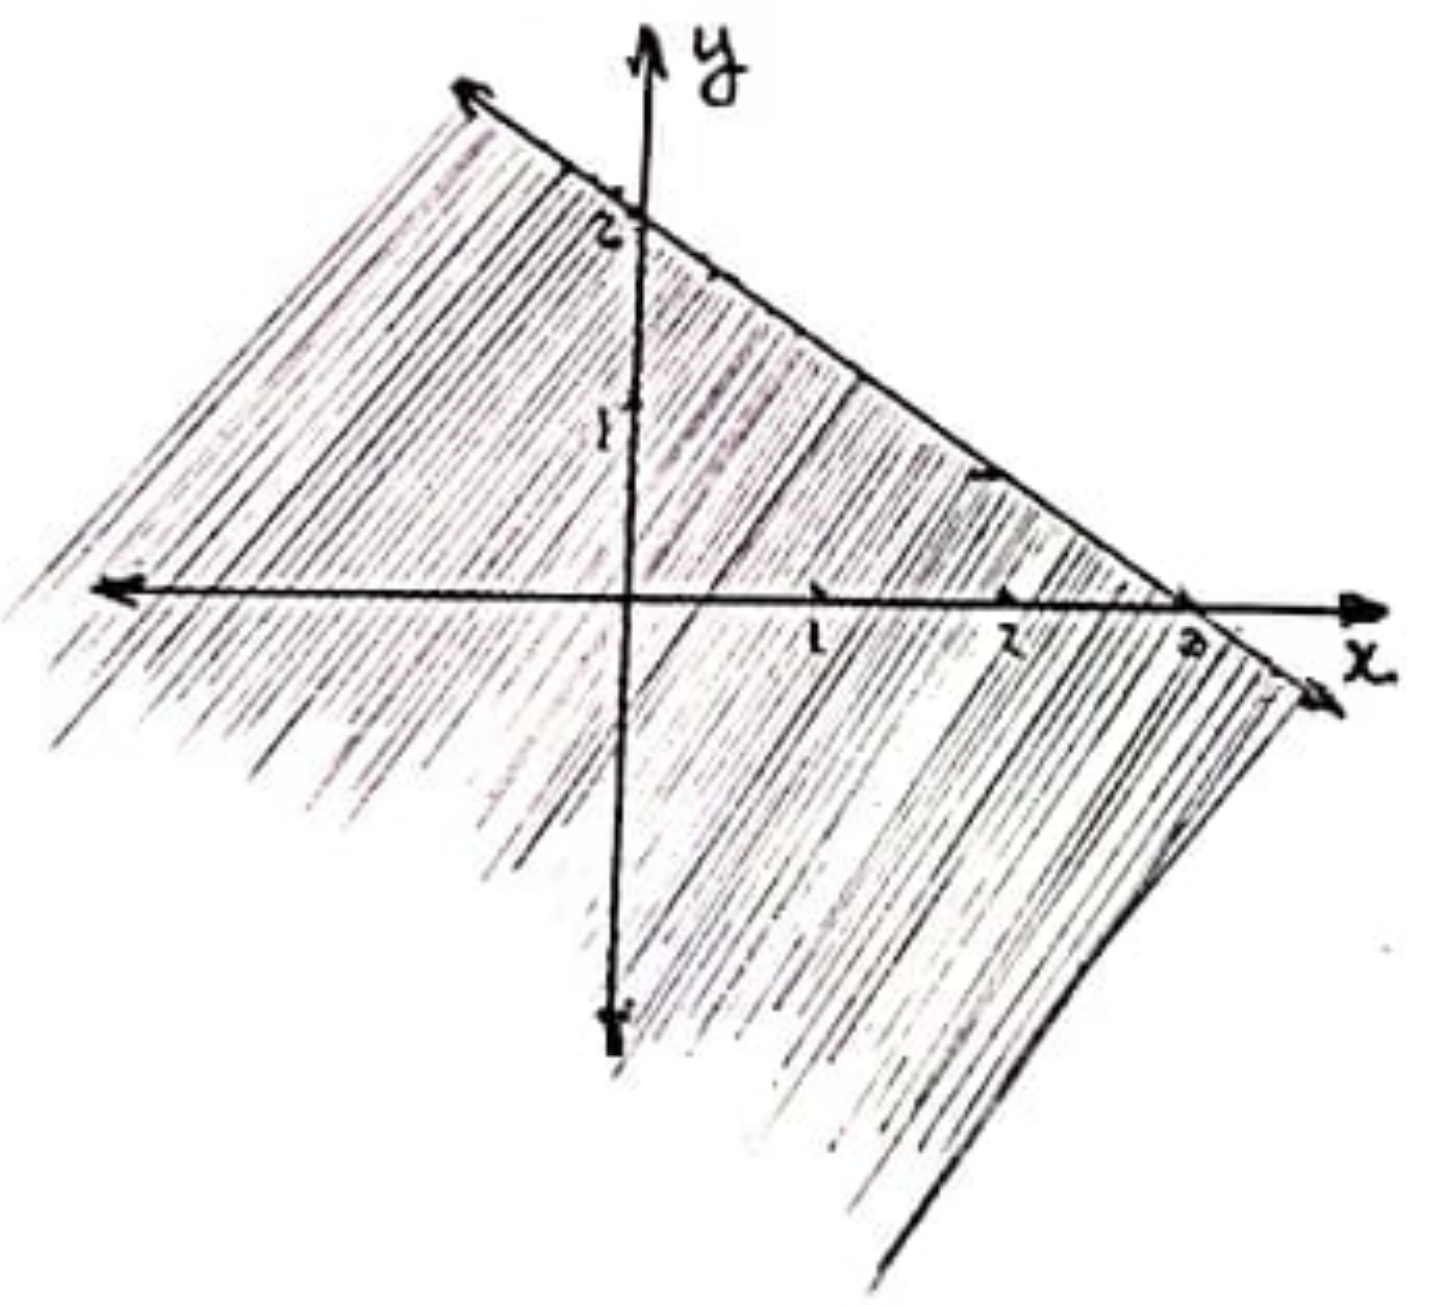
\includegraphics[width = 0.6\linewidth]{plano_simples.png}
  \caption{}
  \label{fig:planoSimples}
\end{figure}

Se $ 2x + 3y \leq 6 $ for em $ \mathbb{R}^{3} $.
A equação $ 2x +3y = 6 $ em $ \mathbb{R}^{3} $ é um plano.
Assim, $ 2x + 3y \leq 6 $ é um semiespaço formado pelo plano e mais os pontos
que estão de um lado do plano, logo, a dimensão do semiespaço é três.